\documentclass[12pt,letterpaper]{article}

\usepackage[utf8]{inputenc}
\usepackage[T1]{fontenc}
\usepackage[brazil]{babel}
\usepackage{lmodern}
\usepackage{amsmath}
\usepackage{amssymb}
\usepackage{booktabs}
\usepackage{geometry}
\usepackage{graphicx}
\usepackage{float}
\usepackage{caption}
\usepackage{subcaption}
\usepackage{siunitx}
\usepackage{microtype}
\usepackage[hidelinks]{hyperref}

\geometry{top=2.5cm,bottom=2.5cm,left=2.7cm,right=2.7cm}
\graphicspath{{figuras_relatorio/}{../Figs/}}
\captionsetup{font=small,labelfont=bf}
\setlength{\parindent}{1.25cm}
\setlength{\parskip}{0.15cm}
\sisetup{output-decimal-marker={,}}

\begin{document}

\pagenumbering{gobble}
\begin{titlepage}
    \centering
    {\Large EEE050\par}
    \vspace{0.4cm}
    {\Large Modelagem e Simulação Multifísica\par}
    \vspace{0.2cm}
    {\large Engenharia de Sistemas -- 2026/02\par}

    \vfill

    {\LARGE\bfseries MODELO DE UM ALTO-FALANTE\par}
    \vspace{0.4cm}
    {\Large Relatório do Trabalho Computacional 02\par}

    \vfill

    {\large\bfseries Autores\par}
    \vspace{0.5cm}
    {\large
    Matheus Carvalho\par
    Talvani de Souza\par
    Gustavo Augusto Ortiz\par
    Gabriel de Araújo\par}

    \vfill

    {\large 30 de agosto de 2026\par}
\end{titlepage}

\pagenumbering{arabic}
\tableofcontents
\newpage

\section{Introdução}

O presente relatório consiste na entrega do segundo trabalho computacional da
disciplina de Modelagem e Simulação Multifísica. O objetivo é modelar e simular
um alto-falante por meio de elementos concentrados, considerando o acoplamento
entre o circuito elétrico da bobina e o movimento mecânico do cone.

O alto-falante é um problema multifísico porque a corrente elétrica que percorre
a bobina produz uma força magnética, responsável pelo deslocamento do conjunto
móvel. Ao mesmo tempo, a velocidade da bobina produz uma força
contraeletromotriz que modifica a corrente do circuito. A posição do cone também
pode alterar o fator de força $Bl$, introduzindo um comportamento não linear.

Os principais componentes considerados na representação do alto-falante são
apresentados na Figura~\ref{fig:componentes}.

\begin{figure}[H]
    \centering
    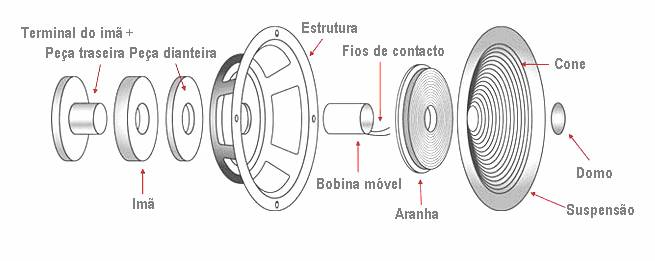
\includegraphics[width=0.72\textwidth]{Aula04_alto-falante_partes.jpg}
    \caption{Principais componentes de um alto-falante. Fonte: adaptado do
    material da Aula 6; imagem original: Novacon~\cite{novacon}.}
    \label{fig:componentes}
\end{figure}

O trabalho é dividido em quatro atividades. Inicialmente é estudada a resposta
do modelo linear a um sinal de voz. Em seguida é construída uma função não
linear para o fator de força. Esse fator é incorporado às equações do sistema e
os resultados dos modelos são comparados. Por fim, os dois modelos são
submetidos a uma entrada senoidal, permitindo separar o comportamento
transitório, verificar o regime periódico alcançado e observar as componentes
espectrais criadas pela não linearidade.

\subsection{Parâmetros e condições iniciais}

Os parâmetros fornecidos no enunciado são apresentados na
Tabela~\ref{tab:parametros}. O sistema parte do repouso, com corrente, posição e
velocidade iniciais nulas.

\begin{table}[H]
    \centering
    \caption{Parâmetros do modelo do alto-falante.}
    \label{tab:parametros}
    \begin{tabular}{clll}
        \toprule
        Símbolo & Grandeza & Valor & Unidade \\
        \midrule
        $m$  & Massa do conjunto móvel & $14{,}35\times10^{-3}$ & kg \\
        $b$  & Coeficiente de amortecimento & $0{,}786$ & kg/s \\
        $k$  & Constante elástica & $1852$ & N/m \\
        $Bl$ & Fator de força nominal & $4{,}95$ & N/A \\
        $L$  & Indutância da bobina & $266\times10^{-6}$ & H \\
        $R$  & Resistência da bobina & $3{,}3$ & $\Omega$ \\
        \bottomrule
    \end{tabular}
\end{table}

As condições iniciais utilizadas em todas as simulações são
\begin{equation}
    i(0)=0,\qquad x(0)=0,\qquad v(0)=0.
    \label{eq:condicoes}
\end{equation}

\subsection{Sinal de entrada}

O arquivo \texttt{TC02-in.wav} contém a voz gravada por um dos integrantes do
grupo. O áudio original é estéreo, possui taxa de amostragem de
\SI{44100}{Hz} e duração de \SI{9.613}{s}, atendendo ao limite de dez segundos.
Como o modelo possui apenas uma entrada de tensão, os dois canais foram
combinados em um sinal mono.

O sinal foi normalizado para um valor de pico inferior a \SI{2}{V}, conforme
solicitado no enunciado, e reamostrado a \SI{12000}{Hz}. Essa taxa é superior à
referência de \SI{9600}{Hz} apresentada no trabalho e reduz o custo
computacional sem eliminar a faixa de frequências de interesse da voz.

\section{Modelagem matemática}

No modelo linear, a tensão aplicada à bobina é dividida entre a queda resistiva,
a tensão no indutor e a força contraeletromotriz produzida pelo movimento da
bobina. A lei de Kirchhoff fornece
\begin{equation}
    u(t)=R i(t)+L\dot{i}(t)+Bl\,\dot{x}(t).
    \label{eq:eletrica}
\end{equation}

O conjunto móvel é representado por uma massa ligada a uma mola e a um
amortecedor viscoso. A força magnética é dada por $Bl\,i(t)$, de modo que
\begin{equation}
    m\ddot{x}(t)=Bl\,i(t)-kx(t)-b\dot{x}(t).
    \label{eq:mecanica}
\end{equation}

Definindo a velocidade $v=\dot{x}$ e o vetor de estados
$\mathbf{z}=[i\;x\;v]^{T}$, as equações governantes podem ser escritas como
\begin{equation}
    \begin{aligned}
        \dot{i} &= -\frac{R}{L}i-\frac{Bl}{L}v+\frac{u}{L},\\
        \dot{x} &= v,\\
        \dot{v} &= \frac{Bl}{m}i-\frac{k}{m}x-\frac{b}{m}v.
    \end{aligned}
    \label{eq:estados}
\end{equation}

No modelo acústico simplificado, considerando a área efetiva do cone e o ponto
de observação fixos, a pressão acústica no campo distante é proporcional à
aceleração do cone. Por esse motivo, a aceleração é utilizada como aproximação
da saída acústica:
\begin{equation}
    \ddot{x}(t)=\frac{Bl}{m}i(t)-\frac{k}{m}x(t)-\frac{b}{m}v(t).
    \label{eq:aceleracao}
\end{equation}

\subsection{Procedimento numérico}

As equações foram integradas com a função \texttt{solve\_ivp} e o método
RK45. A solução é avaliada nos mesmos instantes do áudio, e o maior passo
interno permitido ao integrador é igual a um período de amostragem. Foram
adotadas tolerâncias relativa e absoluta iguais a $10^{-6}$ e $10^{-9}$,
respectivamente.

Como a tensão de entrada está disponível apenas em instantes discretos, o valor
de $u(t)$ solicitado pelo integrador é obtido por interpolação linear entre
amostras consecutivas.

Essa escolha mantém a entrada e a saída sincronizadas e evita que o integrador
atravesse um número excessivo de amostras em um único passo. Os arquivos de
saída são normalizados apenas no momento da gravação do WAV. Os gráficos e os
valores apresentados neste relatório preservam as unidades físicas calculadas
pelo modelo.

\subsection{Procedimento de análise espectral}

Para o cálculo dos espectros, a média de cada sinal é removida e é calculada a
FFT unilateral. Nos sinais de áudio, que não são periódicos no intervalo
observado, é aplicada uma janela de Hann para reduzir o vazamento espectral. As
magnitudes são expressas por
\begin{equation}
    M(f)=20\log_{10}\left(\frac{|X(f)|}{\max |X(f)|}\right).
    \label{eq:espectro}
\end{equation}
Assim, o maior componente de cada curva corresponde a \SI{0}{dB}. Cada sinal é
normalizado separadamente; portanto, os gráficos permitem comparar a
distribuição relativa das componentes, mas não o ganho absoluto entre entrada e
saída. Como a magnitude é normalizada depois da aplicação da janela, não é
necessária uma correção de ganho coerente para essa comparação relativa.

No ensaio senoidal, a FFT é calculada sobre um número inteiro de períodos do
regime periódico e sem janela, evitando espalhamento artificial entre as raias.

\section{Atividade 1 -- modelo linear}

A Figura~\ref{fig:entrada} apresenta a tensão de entrada nos domínios do tempo
e da frequência. A forma de onda possui intervalos de fala separados por
trechos de menor amplitude. O espectro apresenta suas maiores magnitudes nas
baixas e médias frequências, comportamento esperado para uma gravação de voz.

\begin{figure}[H]
    \centering
    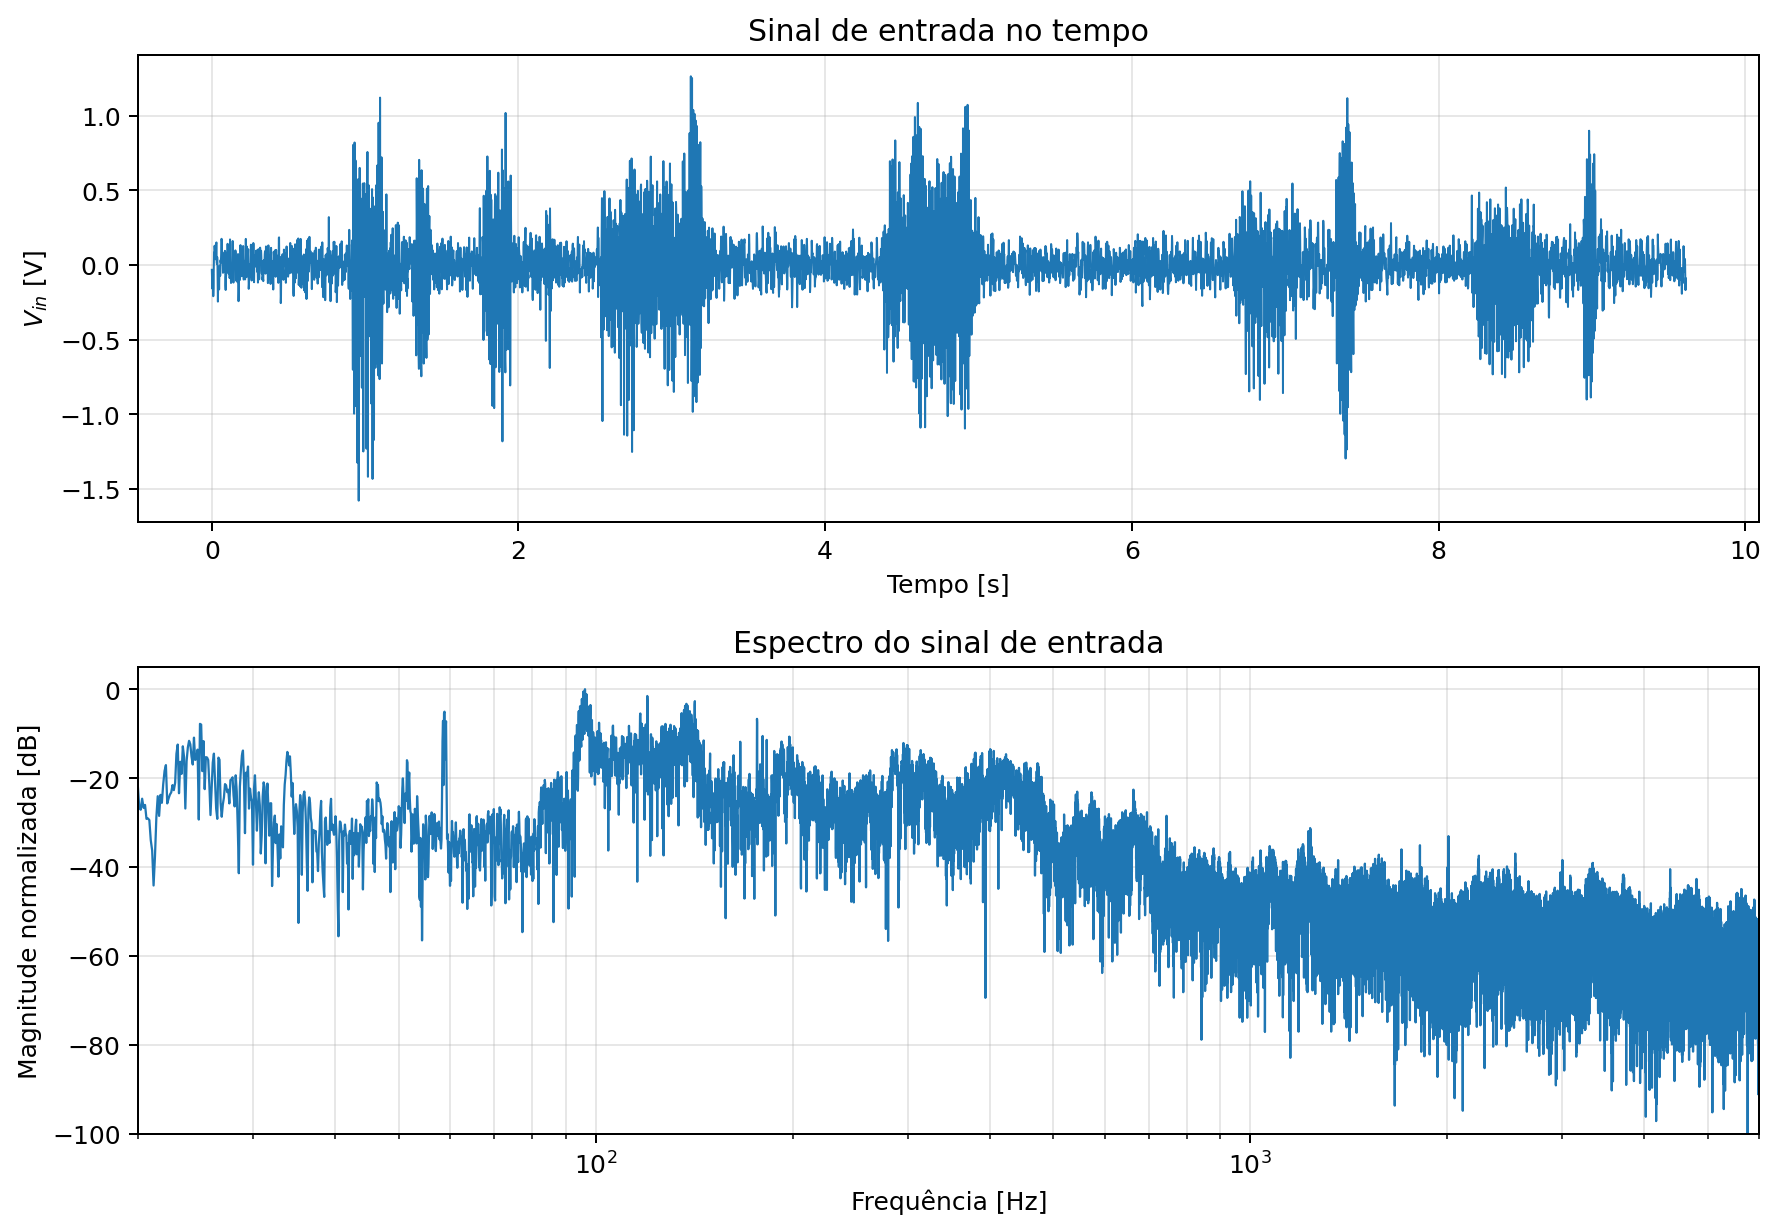
\includegraphics[width=0.92\textwidth]{fig01_entrada.png}
    \caption{Sinal de entrada $V_{in}$ nos domínios do tempo e da frequência.}
    \label{fig:entrada}
\end{figure}

A resposta do modelo linear é mostrada na Figura~\ref{fig:linear}. A corrente
máxima calculada foi de \SI{0.4995}{A}. A excursão máxima do cone foi
$2{,}4159\times10^{-4}$ m, equivalente a aproximadamente \SI{0.242}{mm}, e a
aceleração máxima foi de \SI{176.08}{m/s^2}.

\begin{figure}[H]
    \centering
    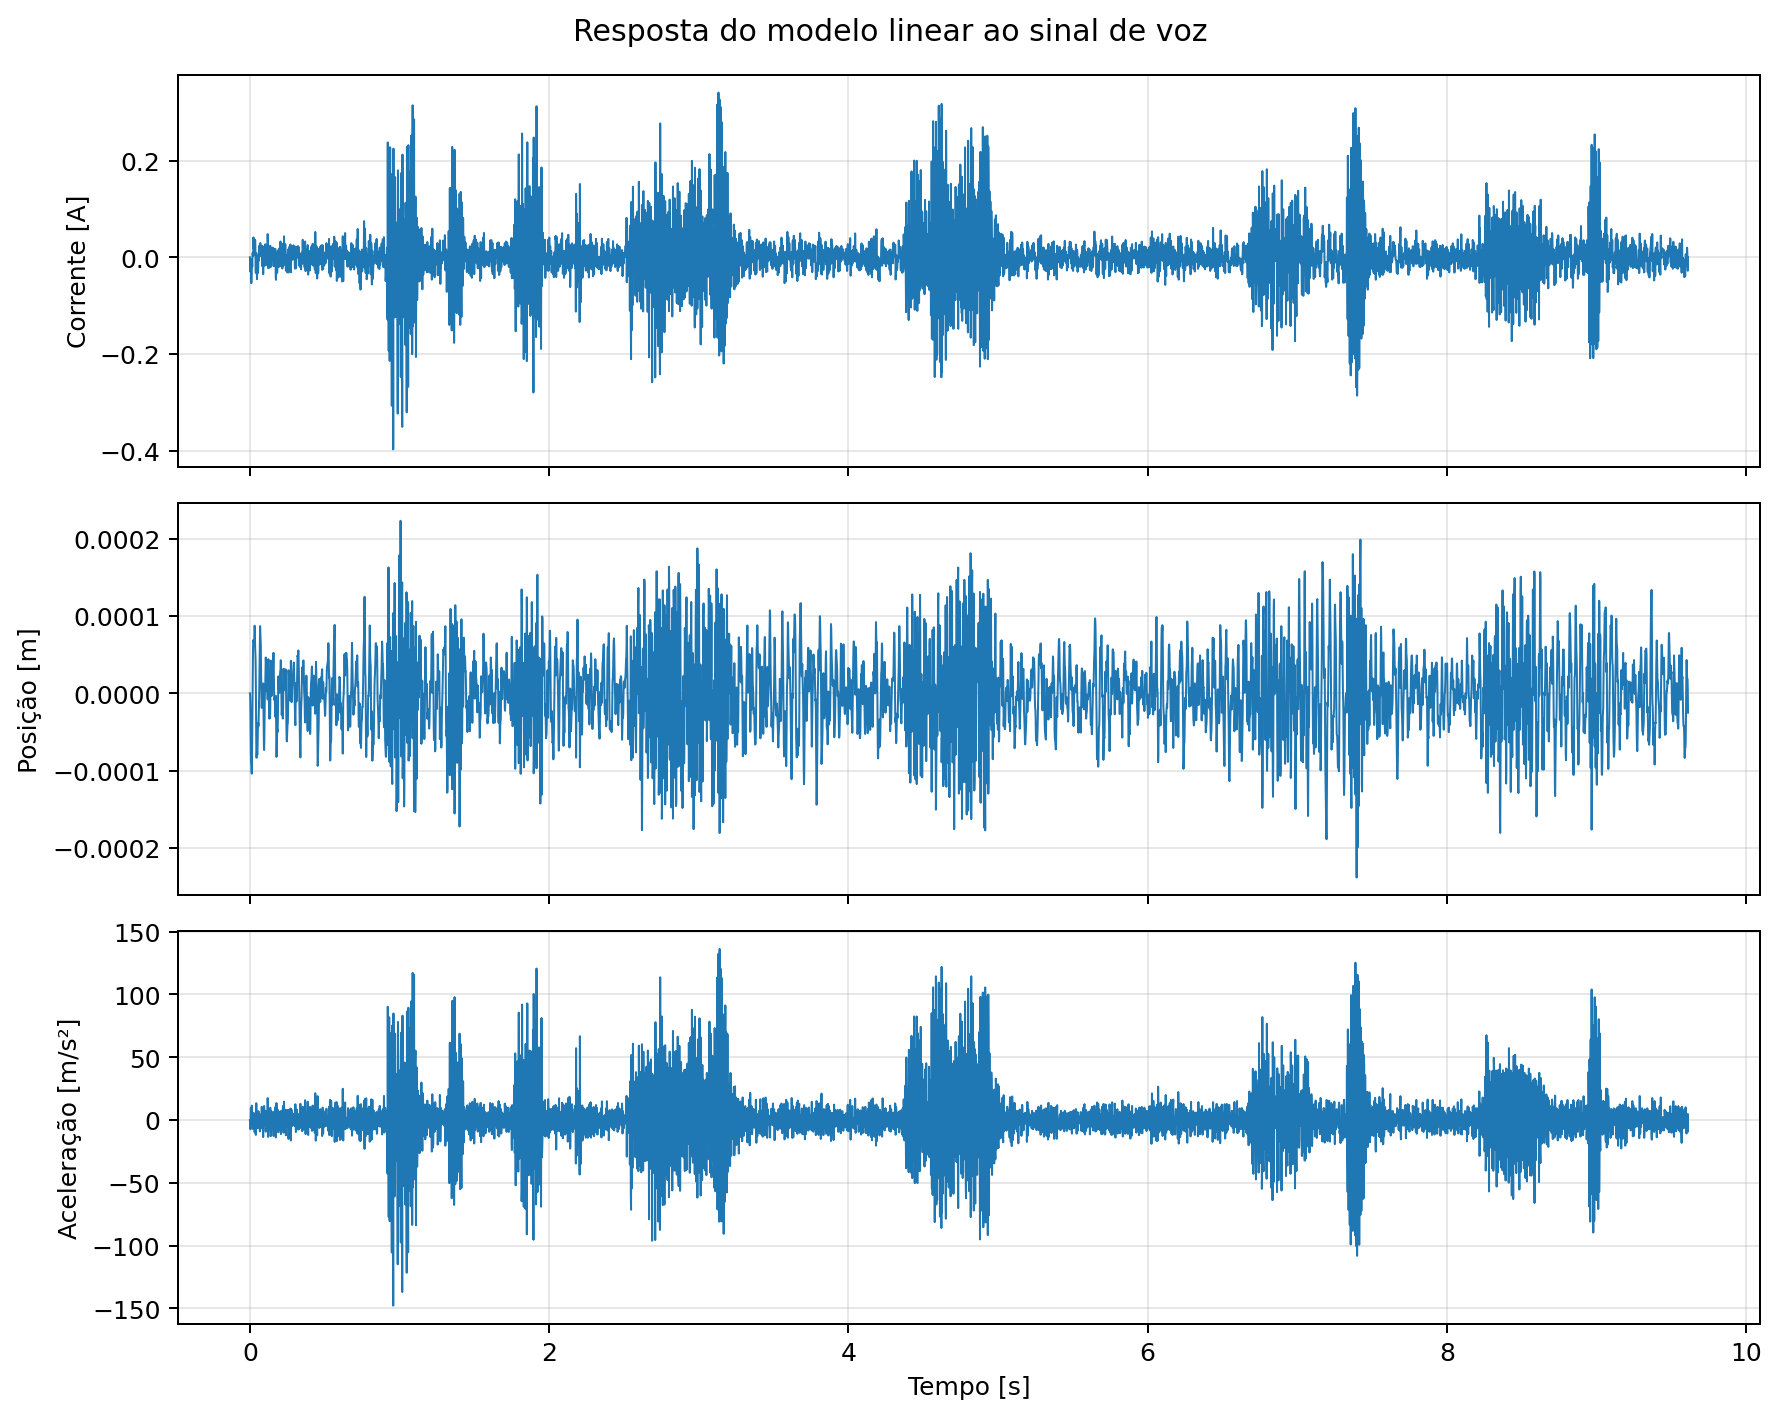
\includegraphics[width=0.92\textwidth]{fig02_modelo_linear.png}
    \caption{Corrente, posição e aceleração do modelo linear para o sinal de voz.}
    \label{fig:linear}
\end{figure}

A Figura~\ref{fig:comparacao-linear} compara a entrada e a aceleração após a
normalização independente de suas amplitudes. Essa normalização é utilizada
apenas para facilitar a comparação visual e não permite calcular o ganho físico
do alto-falante. A saída acompanha a organização temporal do sinal de voz, mas
não é uma cópia da entrada. A resistência e a indutância modificam a corrente,
enquanto a massa, a rigidez e o amortecimento determinam a resposta mecânica.
Consequentemente, o alto-falante reforça algumas faixas e atenua outras.

\begin{figure}[H]
    \centering
    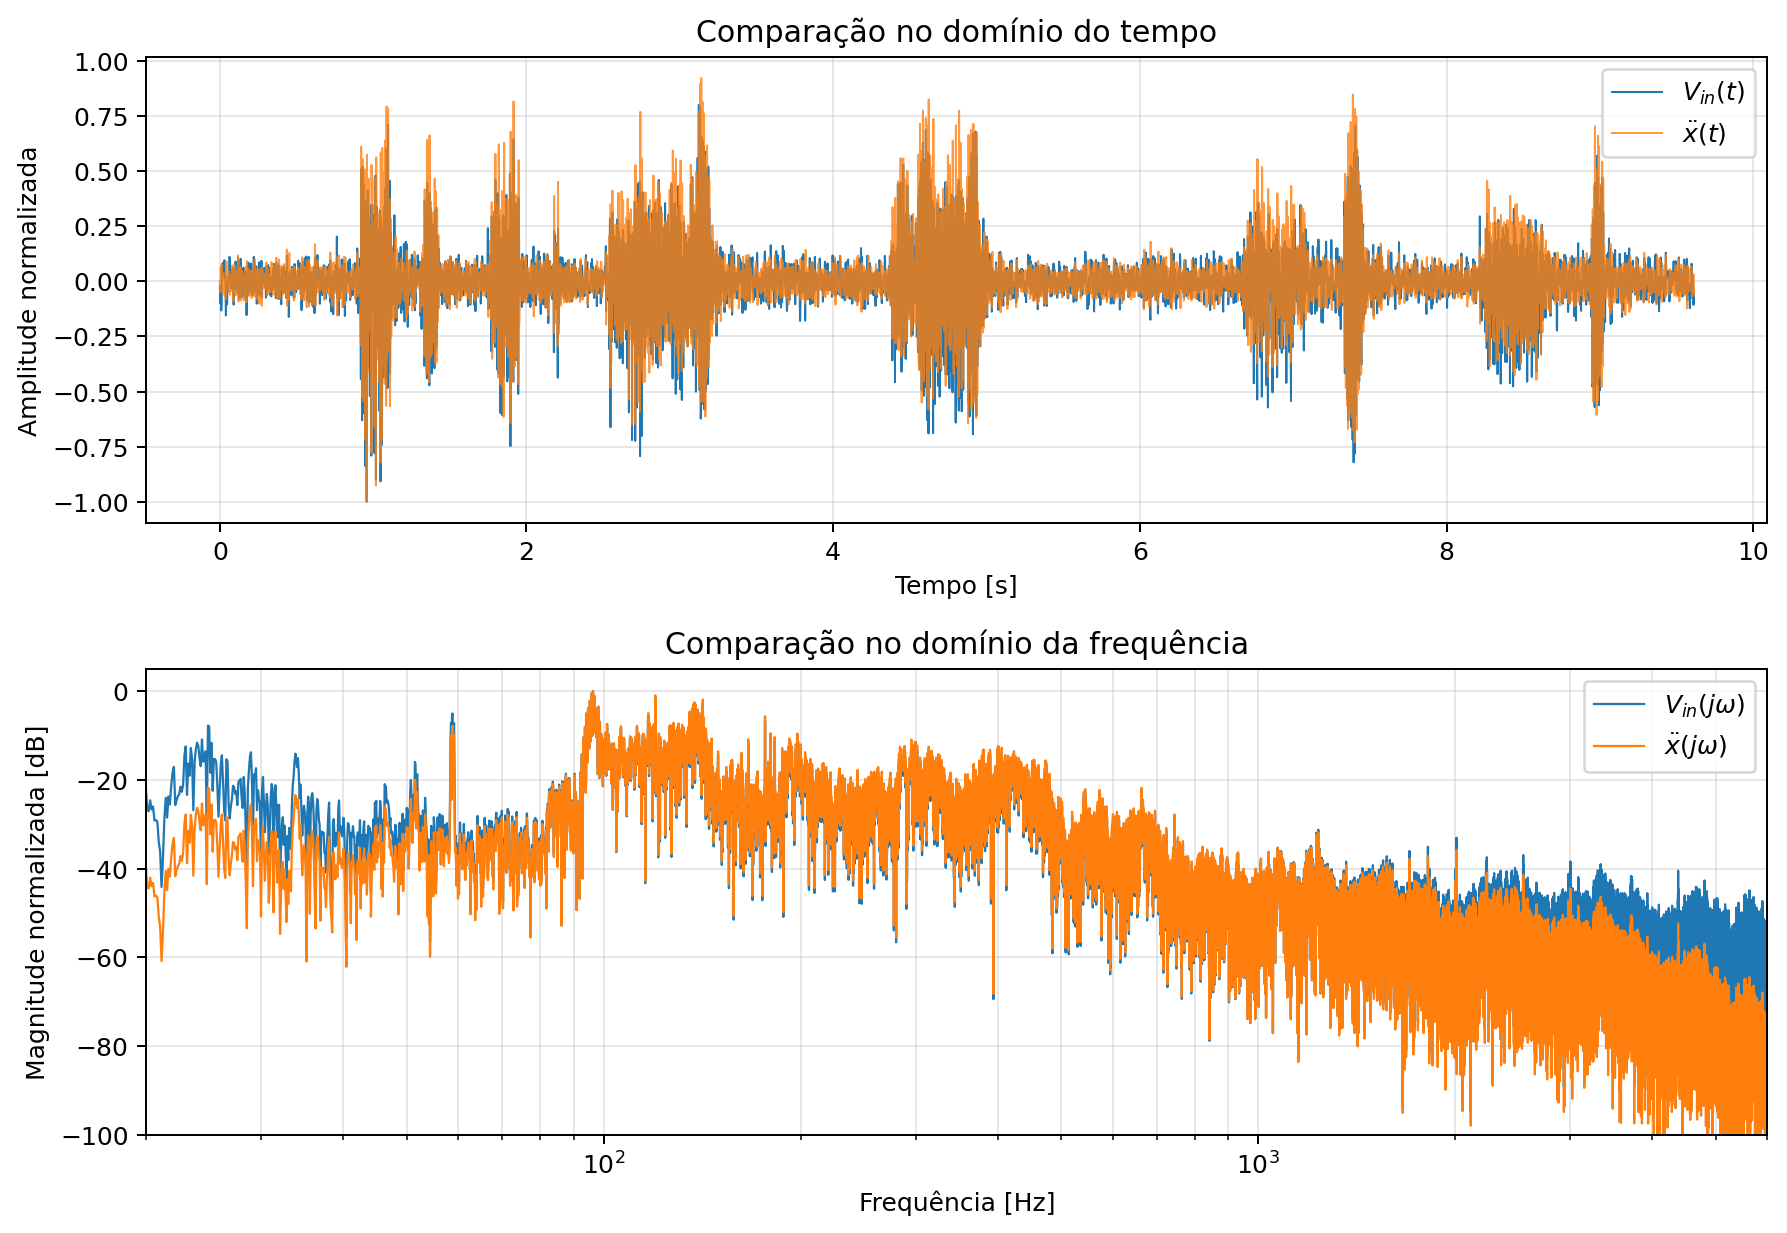
\includegraphics[width=0.92\textwidth]{fig03_comparacao_linear.png}
    \caption{Comparação entre a tensão de entrada e a aceleração do modelo linear.}
    \label{fig:comparacao-linear}
\end{figure}

A aceleração normalizada foi salva no arquivo
\texttt{TC02-out1.wav}, com a mesma duração da entrada.

\section{Atividade 2 -- fator de força não linear}

Para representar a redução da força magnética quando o cone se afasta da
posição de repouso, foram definidos os limites
\begin{equation}
    x_1=0{,}75x_{\max}=1{,}8119\times10^{-4}\ \text{m},
    \qquad
    x_2=1{,}50x_{\max}=3{,}6238\times10^{-4}\ \text{m}.
    \label{eq:limites}
\end{equation}

O fator de força não linear foi construído de forma simétrica:
\begin{equation}
Bl(x)=
\begin{cases}
Bl_0, & |x|\leq x_1,\\[4pt]
Bl_0\left(\dfrac{x_2-|x|}{x_2-x_1}\right)^2,
    & x_1<|x|<x_2,\\[8pt]
0, & |x|\geq x_2.
\end{cases}
\label{eq:bl}
\end{equation}

O polinômio de segunda ordem adotado reproduz qualitativamente a curvatura
indicada no material da Aula 07~\cite{aula6}. A função permanece contínua em
$x_1$ e chega a zero com inclinação nula em $x_2$. Sua derivada, entretanto, é
descontínua em $x_1$. A Figura~\ref{fig:bl} apresenta a curva obtida.

\begin{figure}[H]
    \centering
    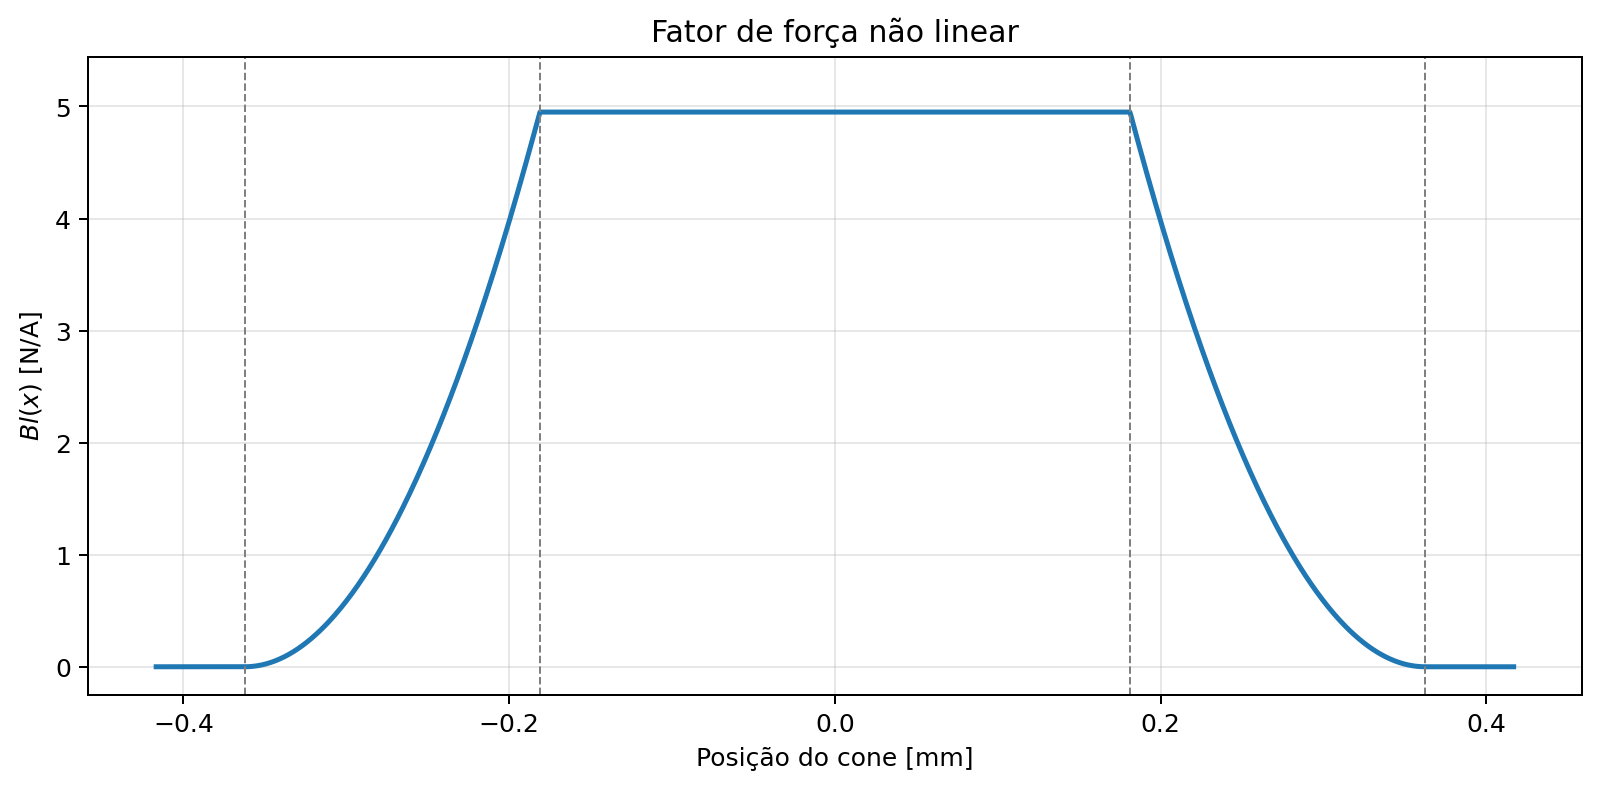
\includegraphics[width=0.88\textwidth]{fig04_fator_forca.png}
    \caption{Fator de força $Bl(x)$ utilizado no modelo não linear.}
    \label{fig:bl}
\end{figure}

\section{Atividade 3 -- avaliação do modelo não linear}

No modelo não linear, o valor constante de $Bl$ foi substituído pela
Equação~\eqref{eq:bl} tanto na equação elétrica quanto na equação mecânica:
\begin{equation}
    \begin{aligned}
        \dot{i} &= \frac{-Ri-Bl(x)v+u}{L},\\
        \dot{x} &= v,\\
        \dot{v} &= \frac{Bl(x)i-kx-bv}{m}.
    \end{aligned}
    \label{eq:naolinear}
\end{equation}

A Figura~\ref{fig:naolinear} apresenta a resposta ao mesmo sinal da
Atividade~1. A maior excursão foi $3{,}7196\times10^{-4}$ m. Esse valor é
ligeiramente maior que $x_2$, de modo que o fator de força chegou
momentaneamente a zero nos maiores deslocamentos.

\begin{figure}[H]
    \centering
    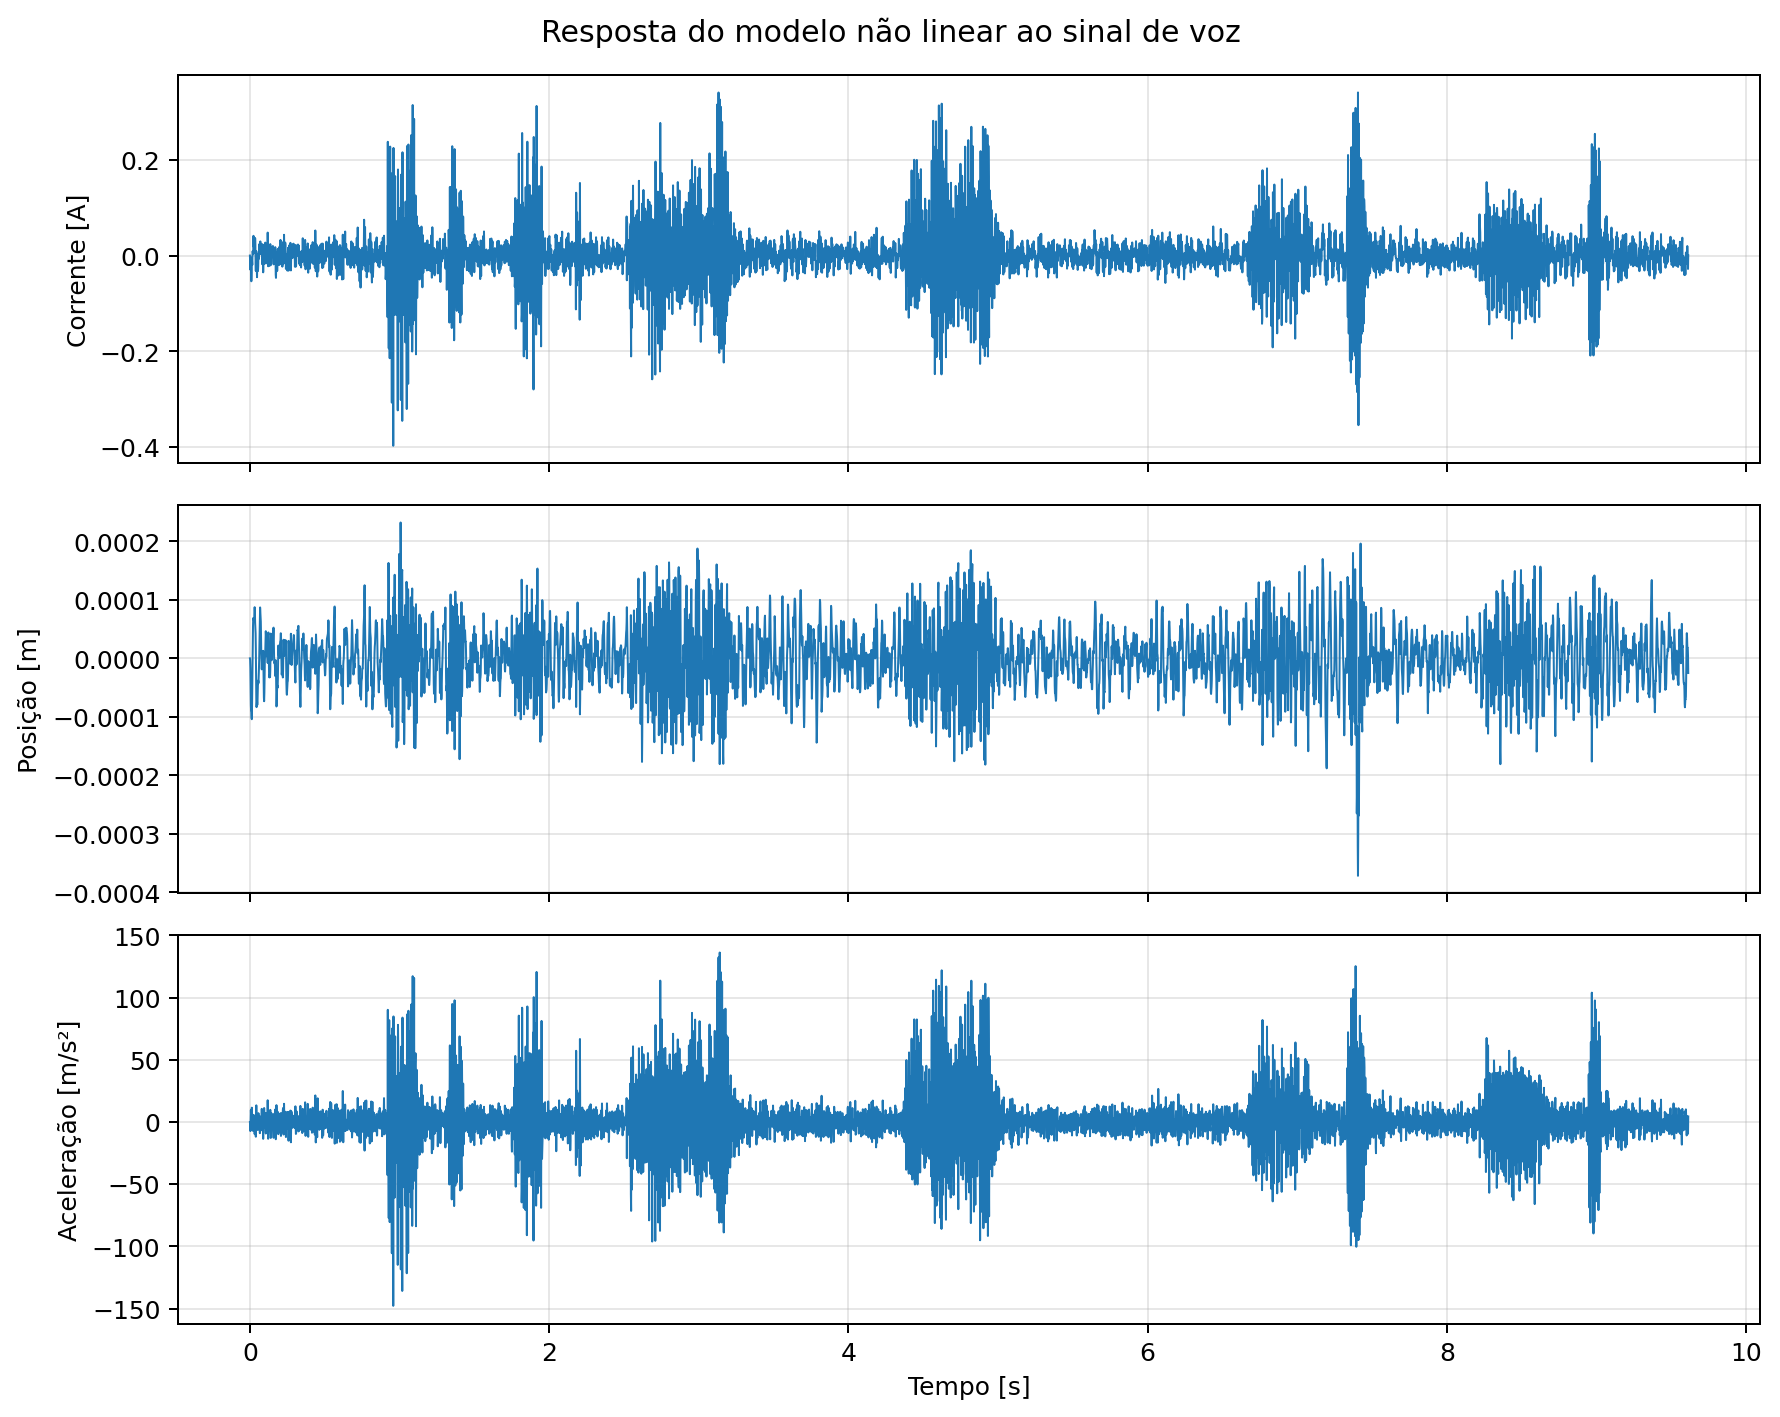
\includegraphics[width=0.92\textwidth]{fig05_modelo_nao_linear.png}
    \caption{Corrente, posição e aceleração do modelo não linear para o sinal de voz.}
    \label{fig:naolinear}
\end{figure}

Na maior parte do áudio, $Bl(x)$ permanece próximo do valor nominal e as
respostas linear e não linear quase se sobrepõem. As maiores diferenças aparecem
nos trechos de maior amplitude, quando o cone ultrapassa $x_1$. A diferença RMS
entre as acelerações foi de \SI{2.0836}{m/s^2}, equivalente a 9,23\% do valor
RMS da aceleração linear. A comparação no tempo e na frequência é apresentada
na Figura~\ref{fig:comparacao-audio}.

\begin{figure}[H]
    \centering
    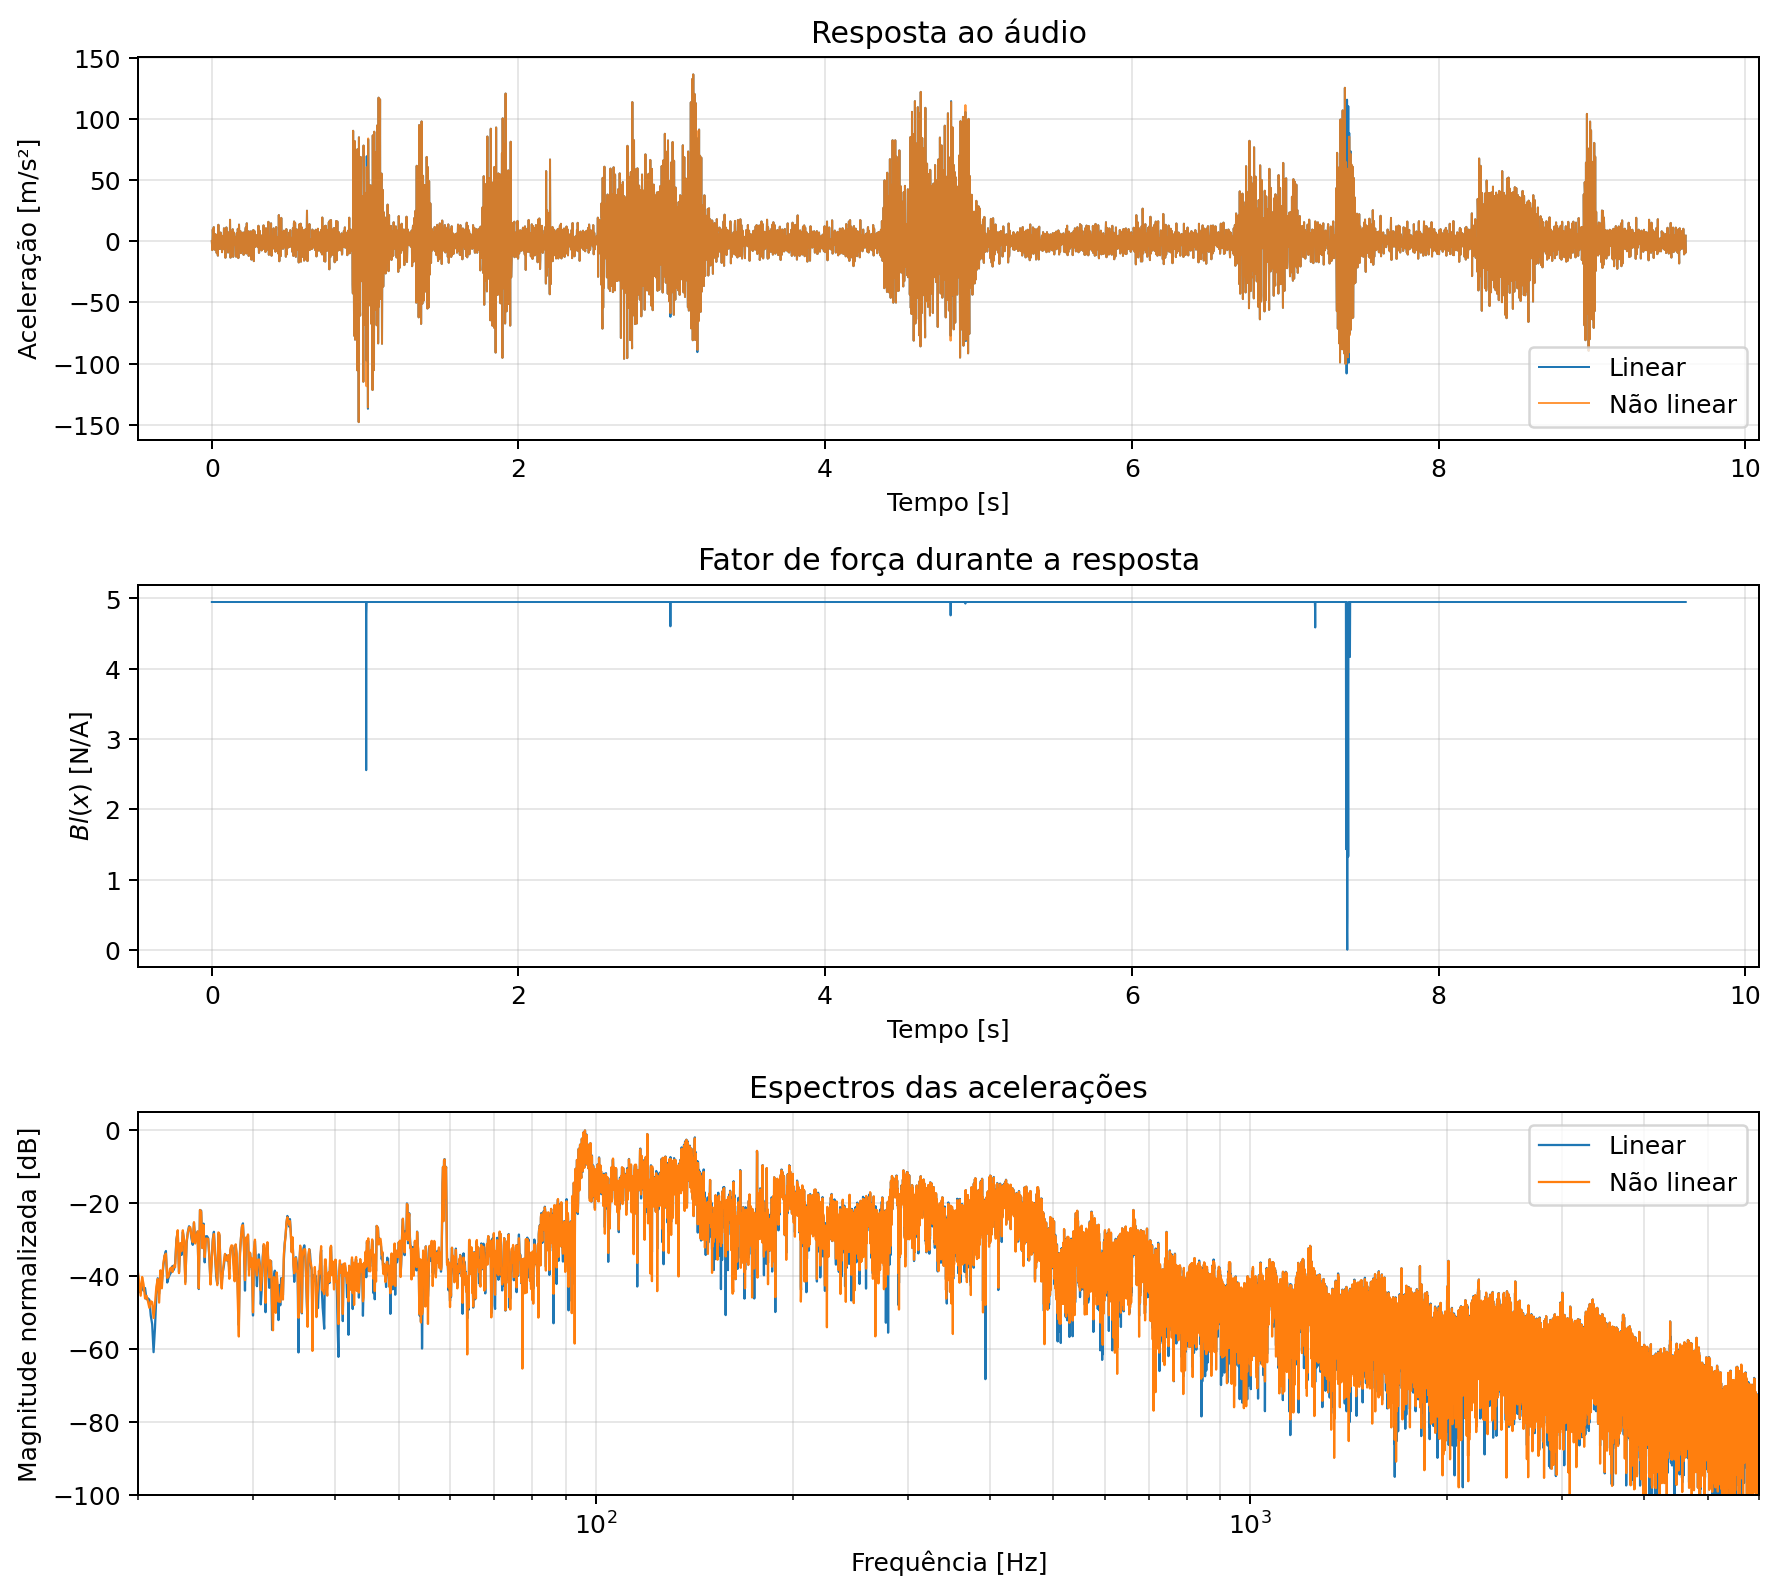
\includegraphics[width=0.92\textwidth]{fig06_comparacao_audio.png}
    \caption{Comparação das respostas linear e não linear ao sinal de voz.}
    \label{fig:comparacao-audio}
\end{figure}

O painel intermediário da Figura~\ref{fig:comparacao-audio} mostra que
$Bl(x)$ permanece em \SI{4.95}{N/A} na maior parte do áudio, mas apresenta
reduções nos picos de deslocamento e chega a zero por um intervalo curto
próximo de \SI{7.4}{s}. Como $Bl(x)$ depende da posição e multiplica a corrente
e a velocidade nas equações governantes, o sistema possui coeficientes
dependentes do estado. Esse acoplamento não linear pode produzir distorção,
mistura de frequências e componentes espectrais ausentes na entrada. A
aceleração normalizada do modelo não linear foi salva em
\texttt{TC02-out2.wav}.

\section{Atividade 4 -- resposta a um sinal senoidal}

Para a última atividade foi escolhida uma frequência de excitação
$f_0=\SI{150}{Hz}$, pertencente à faixa de frequências fundamentais da voz
humana. O sinal possui amplitude de \SI{2}{V}, ou \SI{4}{V} pico a pico, e
duração de 200 períodos:
\begin{equation}
    V_{in}(t)=2\sin(2\pi f_0t),
    \qquad f_0=\SI{150}{Hz}.
    \label{eq:seno}
\end{equation}

Para relacionar o transitório aos parâmetros físicos, calcula-se a frequência
natural não amortecida do subsistema mecânico desacoplado e sua constante de
decaimento:
\begin{equation}
    f_n=\frac{1}{2\pi}\sqrt{\frac{k}{m}}=\SI{57.18}{Hz},
    \qquad
    \tau=\frac{2m}{b}=\SI{36.51}{ms}.
    \label{eq:frequencia-natural}
\end{equation}
Esses valores são referências do sistema massa--mola--amortecedor isolado; o
acoplamento elétrico também modifica o amortecimento e os polos do modelo
completo.

Na Figura~\ref{fig:seno-tempo}, a coluna da esquerda mostra os primeiros cinco
períodos e a coluna da direita mostra os últimos cinco. No modelo linear, a
resposta inicial contém a contribuição natural do sistema, mas converge para
uma resposta periódica praticamente senoidal. A excursão máxima linear foi
$4{,}8168\times10^{-4}$ m.

No modelo não linear, a posição alcançou $6{,}7500\times10^{-4}$ m e ultrapassou
$x_2$. Consequentemente, o fator de força atingiu zero durante parte de alguns
ciclos. A corrente, a posição e principalmente a aceleração apresentam formas
de onda diferentes das obtidas com o modelo linear. A inspeção dos últimos
ciclos também mostra que a resposta não se repete a cada período da entrada.

\begin{figure}[H]
    \centering
    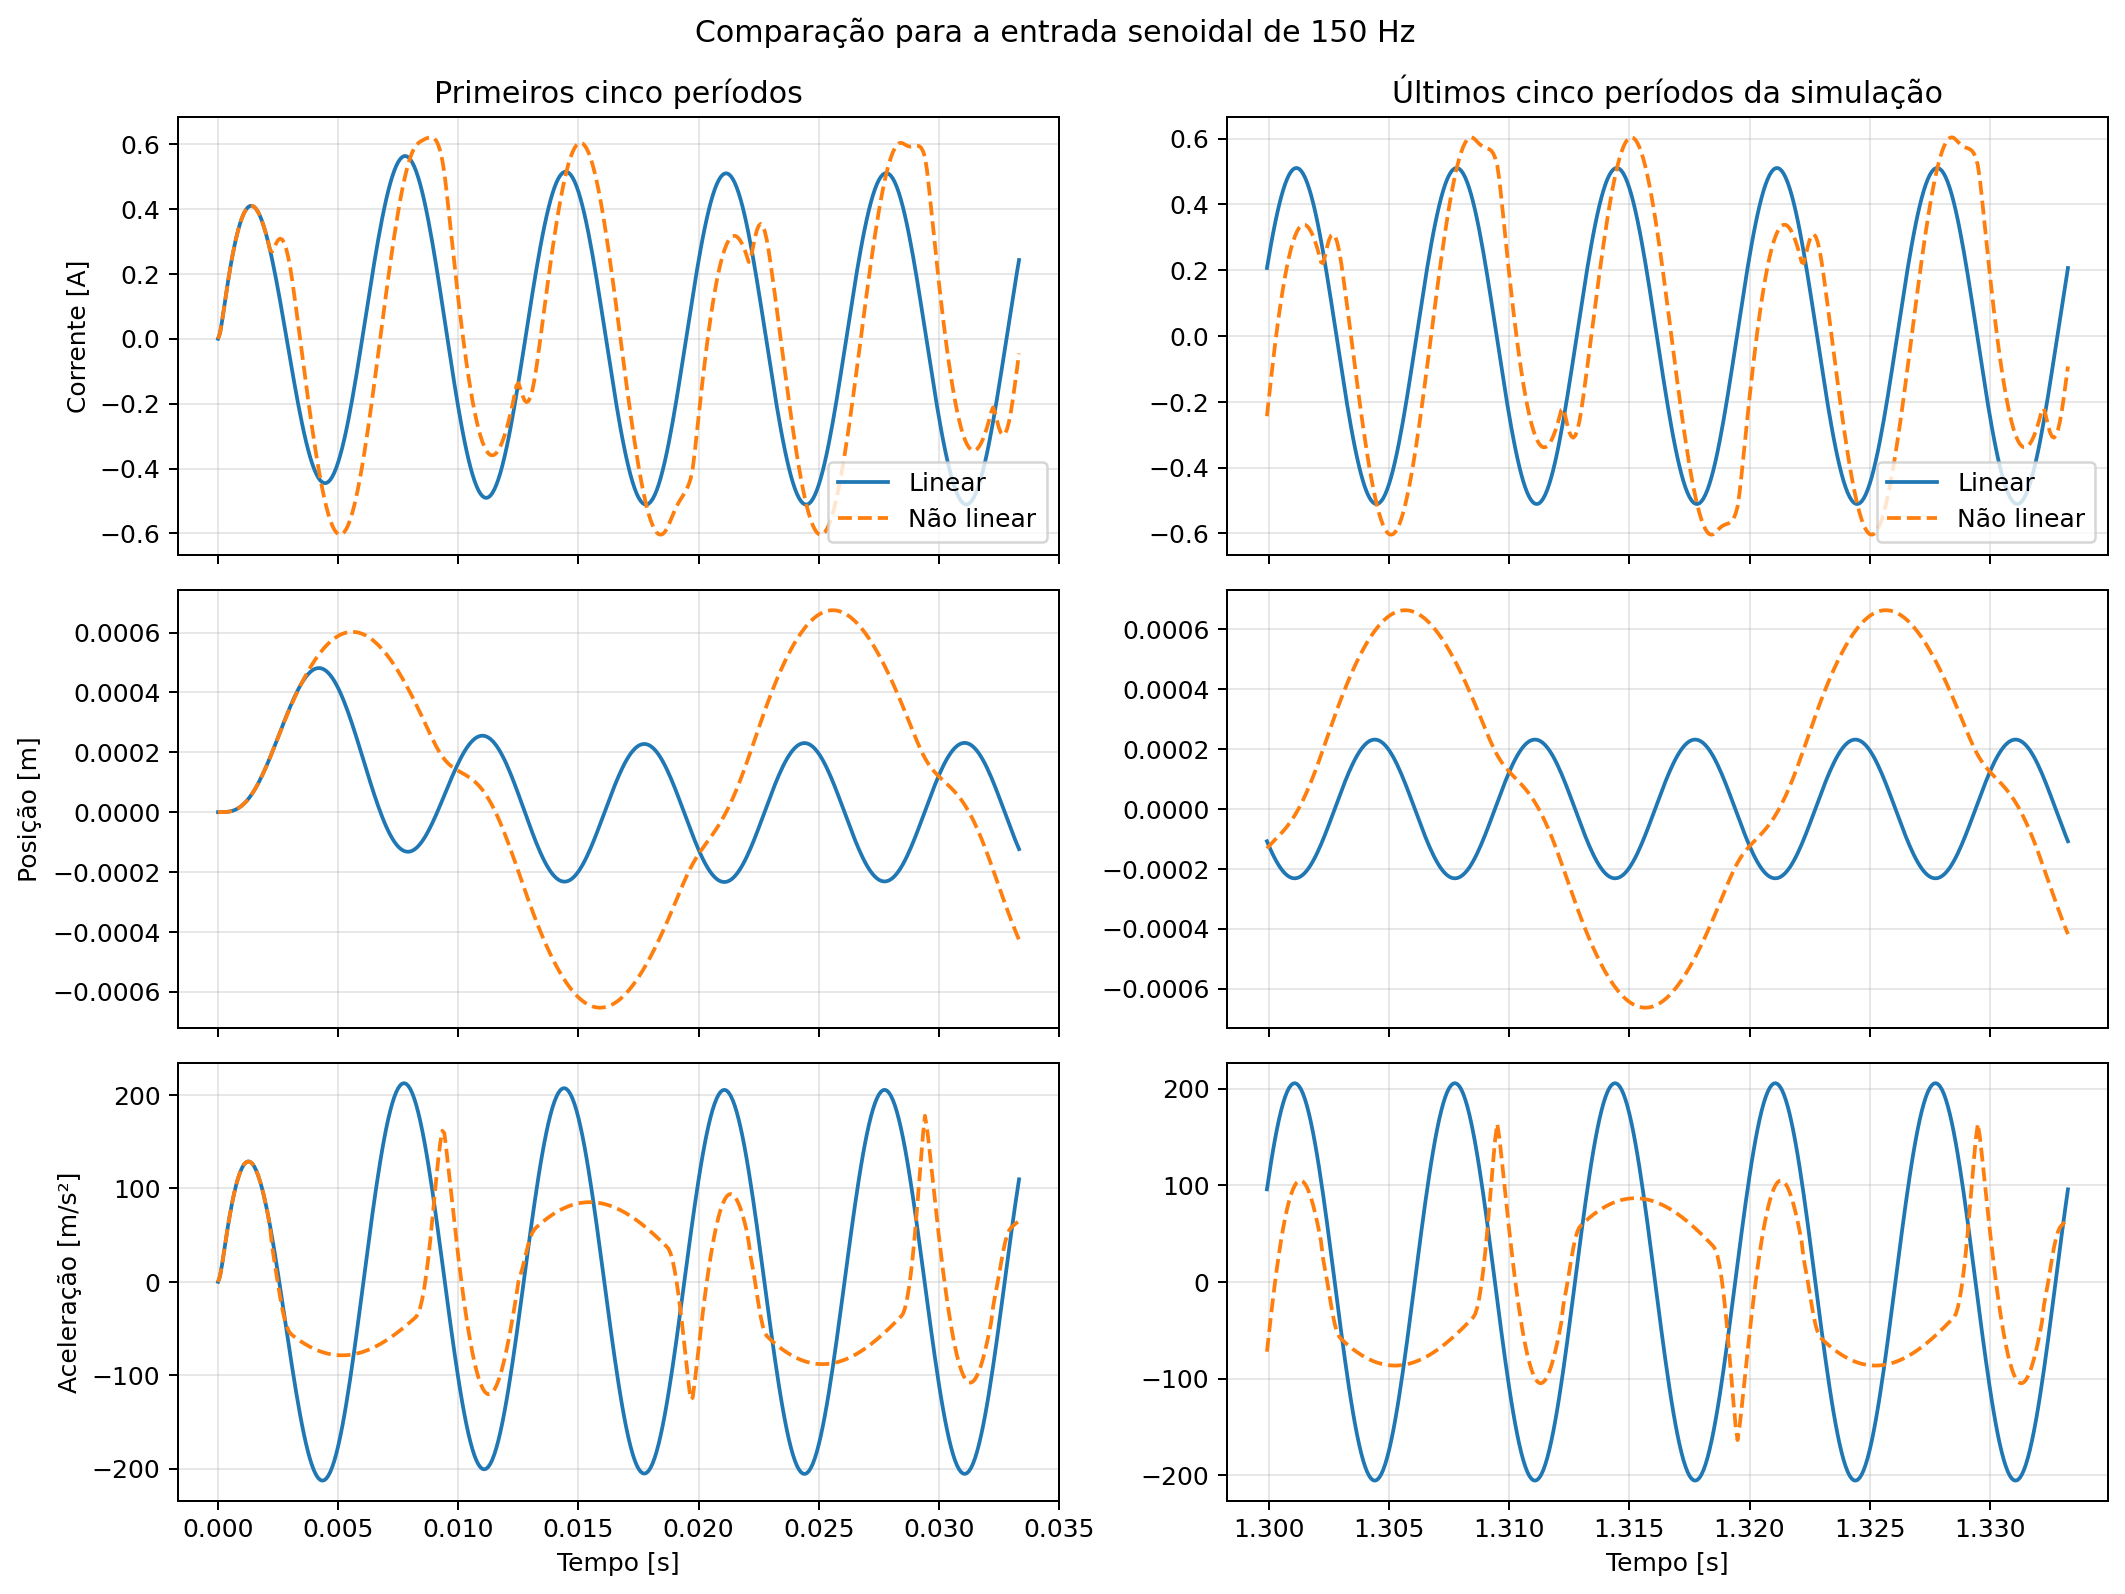
\includegraphics[width=\textwidth]{fig07_senoide_tempo.png}
    \caption{Primeiros e últimos cinco períodos da simulação com entrada de
    \SI{150}{Hz}.}
    \label{fig:seno-tempo}
\end{figure}

\subsection{Verificação do regime periódico}

Para verificar a periodicidade sem depender apenas da inspeção visual, cada
ciclo da aceleração foi comparado com um ciclo anterior. Define-se
\begin{equation}
    e_q(n)=
    \frac{\operatorname{RMS}\!\left(a_n-a_{n-q}\right)}
         {\operatorname{RMS}\!\left(a_n\right)}
    \times 100\%,
    \label{eq:erro-periodicidade}
\end{equation}
em que $a_n$ representa as amostras da aceleração durante o $n$-ésimo período
da entrada e $q$ é o número de períodos de separação.

A Figura~\ref{fig:convergencia} apresenta os erros ao longo dos 200 períodos.
No modelo linear, o erro entre ciclos separados por $T$ converge para
aproximadamente 0,0023\%. No modelo não linear, o erro entre ciclos consecutivos
não converge para zero. Nos ciclos finais, ele oscila entre aproximadamente
129,74\% e 154,71\%, com média de 143,85\%. Em contrapartida, o erro entre
ciclos separados por $3T$ cai para 0,0043\%. A pequena oscilação residual,
também presente no modelo linear, é da ordem do erro numérico da integração.

\begin{figure}[H]
    \centering
    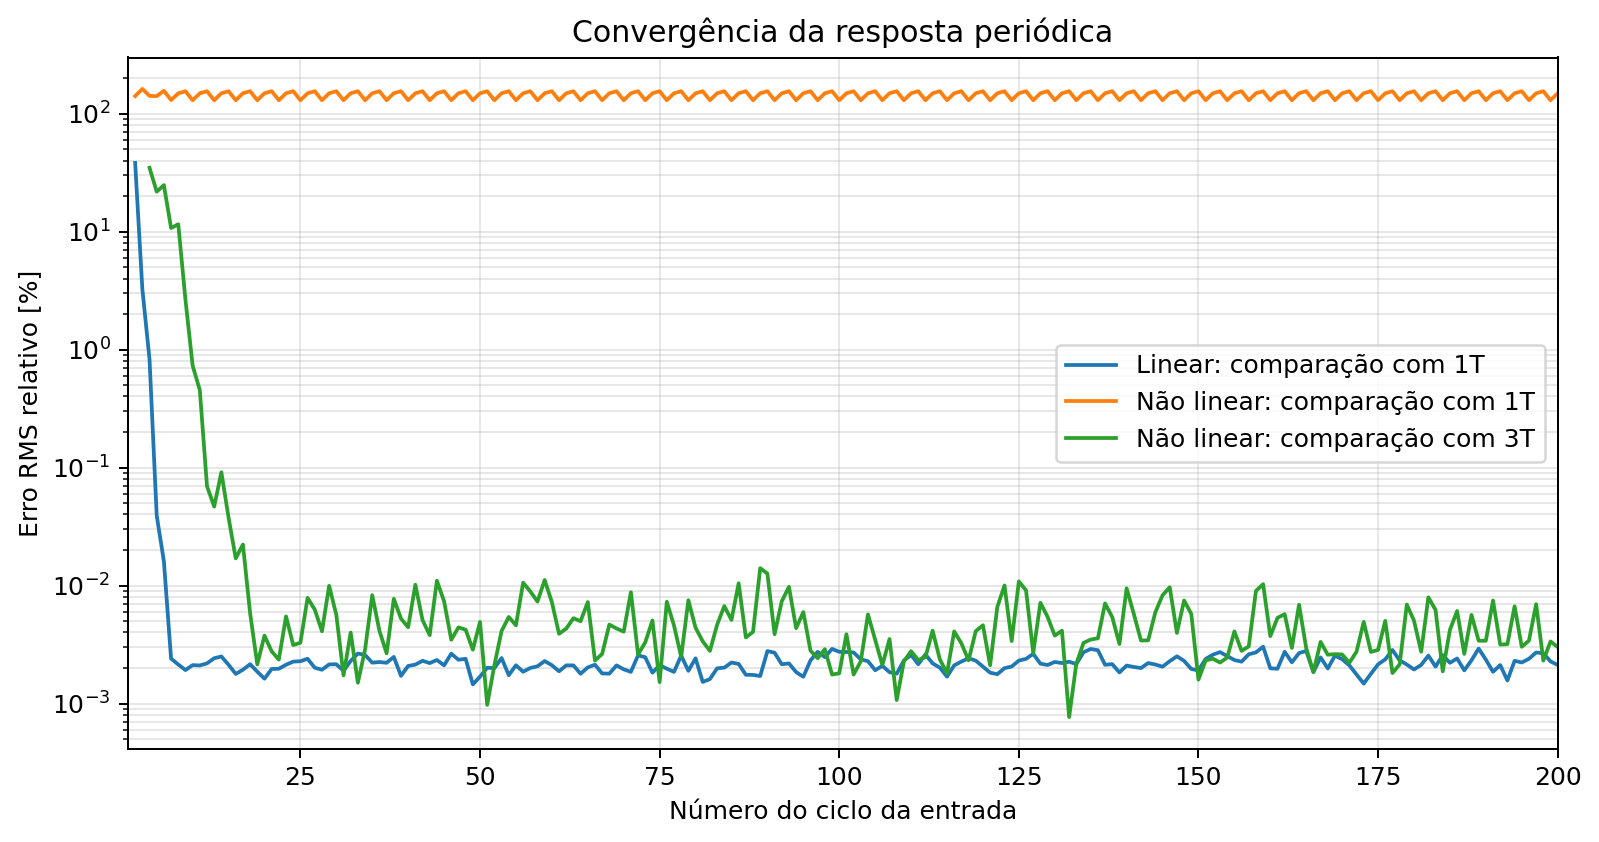
\includegraphics[width=0.9\textwidth]{fig08_convergencia_senoide.png}
    \caption{Erro RMS relativo entre ciclos da resposta senoidal.}
    \label{fig:convergencia}
\end{figure}

Esses resultados demonstram que o modelo linear converge para uma resposta de
período $T$, enquanto o modelo não linear converge para uma órbita periódica de
período $3T$. Portanto, o trecho final pode ser tratado como regime periódico,
mas não possui o mesmo período da excitação.

\subsection{Análise espectral do regime periódico}

A Figura~\ref{fig:seno-espectro} mostra o espectro da aceleração nos últimos 60
períodos da entrada. Esse intervalo corresponde a \SI{0.4}{s}, contém vinte
períodos completos da resposta não linear de período $3T$ e fornece resolução
espectral
\begin{equation}
    \Delta f=\frac{1}{0{,}4}=\SI{2.5}{Hz}.
    \label{eq:resolucao-espectral}
\end{equation}

\begin{figure}[H]
    \centering
    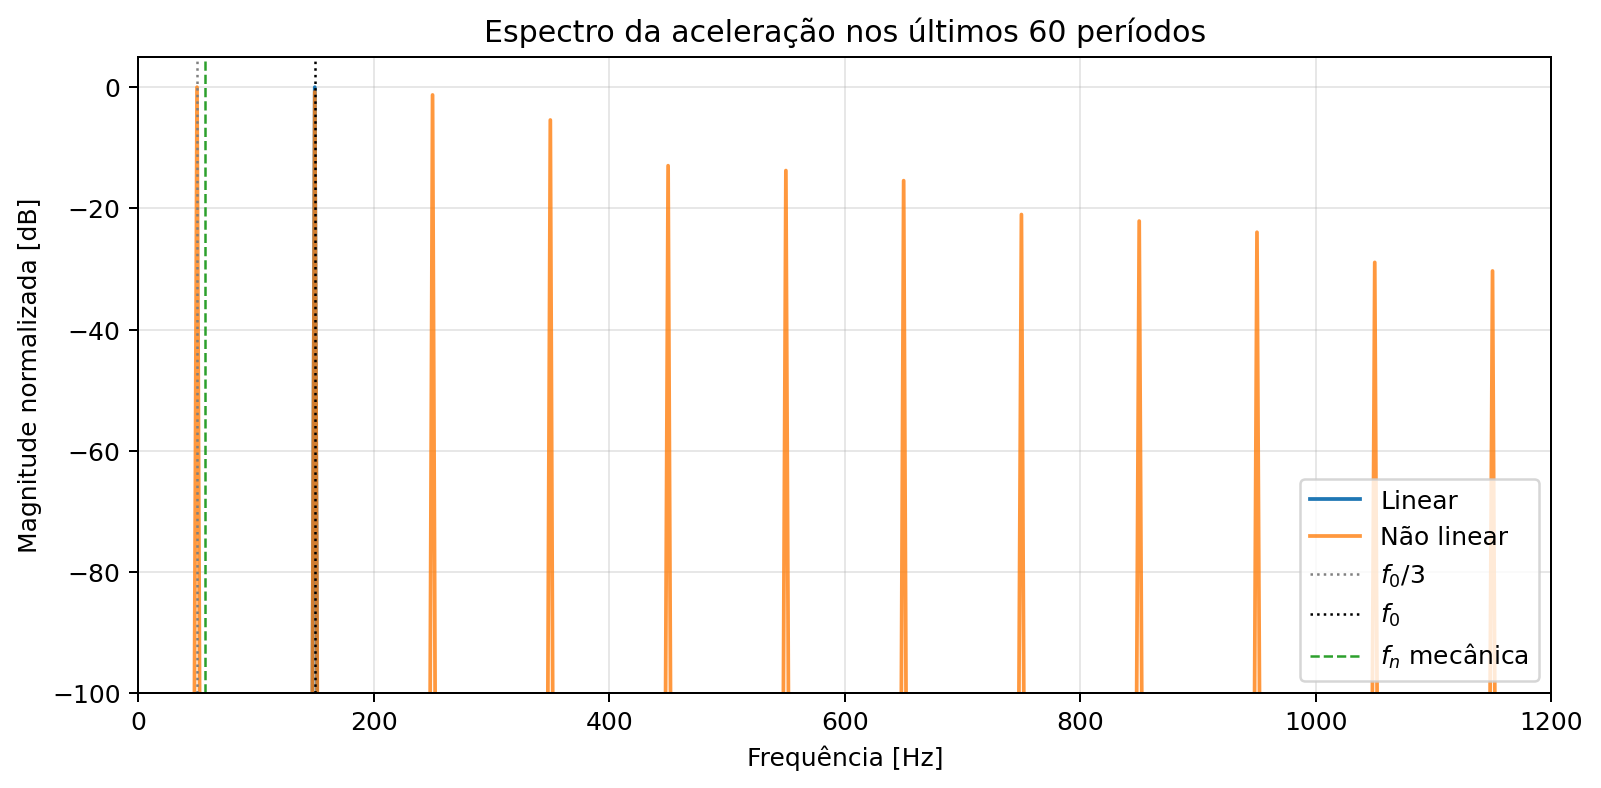
\includegraphics[width=0.9\textwidth]{fig09_senoide_espectro.png}
    \caption{Espectro da aceleração nos últimos 60 períodos da entrada senoidal.}
    \label{fig:seno-espectro}
\end{figure}

No modelo linear, a resposta está concentrada em \SI{150}{Hz}, como esperado.
No modelo não linear, a componente dominante aparece em \SI{50}{Hz},
exatamente $f_0/3$, confirmando a resposta sub-harmônica de ordem 3 observada
na verificação temporal. Essa componente está próxima da frequência natural
mecânica de \SI{57.18}{Hz}, o que pode favorecer sua manifestação, mas a
proximidade não é suficiente para estabelecer uma relação causal.

Também aparecem componentes em \SI{150}{Hz}, \SI{250}{Hz}, \SI{350}{Hz} e
frequências superiores, compatíveis com as harmônicas ímpares da resposta
fundamental de \SI{50}{Hz}. A componente de \SI{450}{Hz}, que também
corresponde à terceira harmônica da excitação, ficou \SI{12.21}{dB} abaixo da
componente de \SI{150}{Hz}. Assim, o modelo não linear não apenas atenua a
entrada: a variação de $Bl(x)$ modifica a forma da onda e cria conteúdo
espectral ausente no modelo linear.

\section{Discussão e conclusão}

\subsection{Discussão dos resultados}

O modelo linear foi capaz de representar a conversão eletromecânica do sinal de
voz com uma implementação simples. A corrente acompanha a tensão aplicada, mas
o movimento do cone é condicionado pela massa, pela rigidez e pelo
amortecimento. Assim, a aceleração mantém a estrutura geral do áudio, porém com
uma distribuição espectral diferente.

A definição correta da curvatura de $Bl(x)$ teve influência direta na intensidade
da não linearidade. Para o sinal de voz, o fator de força permaneceu nominal na
maior parte do tempo e foi reduzido apenas nos picos de deslocamento. Por isso,
as diferenças globais entre os modelos foram pequenas, apesar de localmente
$Bl(x)$ ter atingido zero.

O ensaio senoidal tornou a diferença mais clara. A amplitude de \SI{2}{V}
provocou deslocamentos superiores aos limites calculados a partir do áudio. O
modelo não linear passou a operar repetidamente na região de transição e na
região de força nula, produzindo distorção e novas componentes espectrais. A
simulação longa e o erro de periodicidade mostraram que a resposta não linear
converge para uma órbita de período $3T$, com componente dominante em
\SI{50}{Hz}. Esse resultado mostra que uma entrada senoidal não implica
necessariamente uma saída senoidal com o mesmo período quando os parâmetros do
sistema dependem dos estados.

O modelo continua sendo uma aproximação. Ele considera o cone rígido, ignora
modos estruturais, propagação espacial da onda acústica, variação da indutância,
saturação magnética e outros fenômenos presentes em um alto-falante real. Os
resultados devem, portanto, ser interpretados como tendências do modelo
concentrado adotado.

\subsection{Conclusão}

Conclui-se que o modelo em espaço de estados descreve de forma direta o
acoplamento entre o circuito da bobina e o movimento do cone. Para o sinal de
voz, o modelo linear gerou uma saída coerente com o comportamento esperado de
um sistema eletromecânico seletivo em frequência.

A inclusão do fator de força dependente da posição permitiu representar a perda
de eficiência do atuador para grandes excursões. No áudio, esse efeito ficou
concentrado nos picos de maior amplitude. Na entrada senoidal, a não linearidade
alterou significativamente o transitório e levou o sistema a um regime
periódico sub-harmônico de ordem 3, além de criar novas componentes no espectro.

Os arquivos \texttt{TC02-out1.wav} e \texttt{TC02-out2.wav} registram,
respectivamente, as acelerações normalizadas dos modelos linear e não linear.
O notebook anexado contém a implementação completa, os gráficos e os valores
utilizados neste relatório.

\addcontentsline{toc}{section}{Referências}
\begin{thebibliography}{9}

\bibitem{aula6}
ADRIANO, Ricardo.
\textit{Aula 06 -- Modelagem de um alto-falante e Aula 07 -- Trabalho
Computacional 02}.
Material da disciplina Modelagem e Simulação Multifísica, UFMG, 2026.

\bibitem{novacon}
NOVACON.
\textit{Alto-falantes: componentes e funcionamento}.
Disponível em: \url{http://www.novacon.com.br/audioafca.htm}.
Acesso em: 30 ago. 2026.

\end{thebibliography}

\end{document}
